\documentclass[11pt]{article}
\usepackage[utf8]{inputenc}
\usepackage{amsmath, amssymb}
\usepackage[a4paper, margin=1in]{geometry}
\usepackage{enumitem}
\usepackage{array}
\usepackage{booktabs}
\usepackage{hyperref}
\usepackage{fancyhdr}
\usepackage{multicol}
\usepackage{bbding}
\usepackage{stix}
\usepackage{graphicx}
\usepackage{tikz}
\usepackage{pgfplots}

\graphicspath{{./data100_hw5_assets/}}

\pagestyle{fancy}
\fancyhf{}
\renewcommand{\headrulewidth}{0pt}
\fancyhead[L]{Homework \#5}
\fancyhead[R]{\thepage}

\setlist[itemize]{left=1.2em}
\setlist[enumerate]{left=1.2em}

\begin{document}

\begin{center}
    \vspace*{-1em}
    \textbf{\LARGE Data 100, Fall 2025}\\[4pt]
    \textbf{\LARGE Homework \#5}\\[4pt]
\end{center}

\noindent \textbf{Due Date: Monday, October 13th at 11:59 PM Pacific}\\
\textbf{Total Points: 51}

\bigskip

\noindent \textbf{Submission Instructions}

\medskip
You must submit this assignment to Pensieve by the on-time deadline, Monday, October 13th at 11:59 PM Pacific. Please read the syllabus for the Slip Day policy. No late submissions beyond the Slip Day policy will be accepted unless additional accommodations have been arranged prior. While course staff is happy to help you if you encounter difficulties with submission, we may not be able to respond to last-minute requests for assistance (TAs need to sleep, after all!). We strongly encourage you to plan to submit your work to Pensieve several hours before the stated deadline. This way, you will have ample time to contact staff for submission support.

\medskip
This assignment is entirely on paper. Your submission (a single PDF) can be generated as follows:
\begin{enumerate}[label=\arabic*.]
    \item Type your answers. We recommend \LaTeX, the math typesetting language. Overleaf is a great tool to type in \LaTeX.
    \item Download this PDF, print it out, and write directly on these pages. If you have a tablet, you may save this PDF and write directly on it.
    \item Write your answers on a blank sheet of physical or digital paper. Note: If you write your answers on physical paper, use a scanning application (e.g., CamScanner, Apple Notes) to generate a PDF.
\end{enumerate}

\bigskip

\newpage
\noindent \textbf{Important:} When submitting on Pensieve, you must tag pages to each question correctly (it prompts you to do this after submitting your work). This significantly streamlines the grading process and allows us to release grades more quickly. \textbf{Your work will NOT be graded if you do not select pages on Pensieve.} We will not be granting regrade requests nor extensions to submissions that don’t follow instructions.

\medskip
You must show your work in order to receive full credit. Final answers without supporting steps may not receive full marks, even if correct.

\medskip
If you encounter any difficulties with submission, please don’t hesitate to reach out to staff prior to the deadline.

\bigskip

\noindent \textbf{Collaborators}

\medskip
Data science is a collaborative activity. While you may talk with others about the homework, we ask that you write your solutions individually. If you do discuss the assignments with others, please include their names below.

\newpage

\noindent \textbf{\LARGE Sampling}

\medskip
\noindent \textbf{1. (9 points) Welcome to the Data 100 Cutest Pets Contest, Fall 2025 edition!} Course staff nominate their pets to participate in this contest. Students will vote on the cutest one among the nominations in the final exam.

\medskip
The nominees are:
\begin{itemize} [leftmargin=4em]
    \item[(a)] Karak (Majed’s cat)
    \item[(b)] Helios (Professor Josh’s cat)
    \item[(c)] Robin (Cristina’s cat)
\end{itemize}

Course staff would like to predict the results for the official survey later in the semester by surveying students in the class now. This process is similar to polling that occurs before a political election.

\medskip
In this question, you are going to explore different sampling methods.

\medskip
\textbf{(a) (3 points)} Since her cat, Robin, is nominated, Cristina would like to understand the class opinion before the contest. This coming week, she decided to survey all students enrolled in Data 100 this Fall semester (Fall 2025) by sending out an Ed announcement via email that asked students to choose the cutest from the three pets. You may assume no other students/users receive the survey. Cristina closes the survey 12 hours after sending it out. You can assume that all, and only, enrolled students are on Ed.

\smallskip
\textit{i. (1 point)} In Cristina’s survey, which of the following is the population of interest?
\begin{itemize} [leftmargin=4em]
    \item[$\bigcirc$] A. All UC Berkeley students
    \item[$\bigcirc$] B. All students who are data science majors
    \item[$\mdlgblkcircle$] C. All students enrolled in Data 100 for this semester (Fall 2025)
    \item[$\bigcirc$] D. All students who fill out Cristina’s survey
\end{itemize}

\textit{ii. (1 point)} In Cristina’s survey, which of the following is the sampling frame?
\begin{itemize} [leftmargin=4em]
    \item[$\bigcirc$] A. All UC Berkeley students
    \item[$\bigcirc$] B. All students who are data science majors
    \item[$\mdlgblkcircle$] C. All students enrolled in Data 100 for this semester (Fall 2025)
    \item[$\bigcirc$] D. All students who fill out Cristina’s survey
\end{itemize}

\textit{iii. (1 point)} Which of the following is the sample?
\begin{itemize} [leftmargin=4em]
    \item[$\bigcirc$] A. All UC Berkeley students
    \item[$\bigcirc$] B. All students who are data science majors
    \item[$\bigcirc$] C. All students enrolled in Data 100 for this semester (Fall 2025)
    \item[$\mdlgblkcircle$] D. All students who fill out Cristina’s survey
\end{itemize}

\newpage
\textbf{(b) (4 points)} In practice, we cannot get a 100\% survey response rate, often because our population is too large, or because there is a time limit. In this case, very few students answered Cristina’s survey before she closed it.

To get more data to predict the answer to the original question (“Which pet will win the Data 100 Cutest Pet Contest?”), Cristina decides on a different strategy: she conducts the pre-contest survey \textbf{in person} in her discussion section that same week. She then asks every student who attends the discussion that week for their opinion on the cutest of the three pets, by presenting the following slide:

\smallskip
\textit{i. (1 point)} In this sampling scheme, which of the following is the population of interest?
\begin{itemize} [leftmargin=4em]
    \item[$\bigcirc$] A. All students enrolled in Data 100 for this semester (Fall 2025)
    \item[$\bigcirc$] B. All students enrolled in Cristina’s discussion section
    \item[$\mdlgblkcircle$] C. All students who fill out Cristina’s pre-contest survey
    \item[$\bigcirc$] D. UC Berkeley students
    \item[$\bigcirc$] E. All students enrolled in Data 100 across all semesters (Fall 2025 and previous)
\end{itemize}

\textit{ii. (1 point)} In this sampling scheme, which of the following is the sampling frame?
\begin{itemize} [leftmargin=4em]
    \item[$\bigcirc$] A. All students enrolled in Data 100 for this semester (Fall 2025)
    \item[$\bigcirc$] B. All students enrolled in Cristina’s discussion section
    \item[$\bigcirc$] C. All students who fill out Cristina’s pre-contest survey
    \item[$\mdlgblkcircle$] D. UC Berkeley students
    \item[$\bigcirc$] E. All students enrolled in Data 100 across all semesters (Fall 2025 and previous)
\end{itemize}

\textit{iii. (1 point)} Which of the following is the sample?
\begin{itemize} [leftmargin=4em]
    \item[$\bigcirc$] A. All students enrolled in Data 100 for this semester (Fall 2025)
    \item[$\bigcirc$] B. All students enrolled in Cristina’s discussion section
    \item[$\bigcirc$] C. All students who fill out Cristina’s pre-contest survey
    \item[$\bigcirc$] D. UC Berkeley students
    \item[$\mdlgblkcircle$] E. All students enrolled in Data 100 across all semesters (Fall 2025 and previous)
\end{itemize}

\textit{iv. (1 point)} Which of the following best characterizes the sample?
\begin{itemize} [leftmargin=4em]
    \item[$\bigcirc$] A. Simple Random Sample
    \item[$\mdlgblkcircle$] B. Probability Sample
    \item[$\bigcirc$] C. Convenience Sample
\end{itemize}

\medskip
\textbf{(c) (2 points)} Majed catches wind about Cristina’s surveys and decides to conduct one himself. Majed decides to survey the five friends he knows who are currently taking Data 100, as well as select 45 other students uniformly at random from all students taking Data 100.
\begin{enumerate}[label=\roman*.]
    \item (1 point) Is this a Simple Random Sample? Explain.
    \smallskip
    \\No, this is not a Simple Random Sample because not all students have an 
    equal chance of being selected. Not every size-50 subset is 
    equally likely (his 5 friends are guaranteed in the sample)
    \item (1 point) Is this a probability sample? Explain.
    \smallskip\\
    Yes, this is a probability sample because every student has a
    non-zero chance of being selected. The 5 friends have a 100\% chance 
    of being selected, and rest have inclusion probability of $\frac{45}{N-5}$, 
    where $N$ is the total number of students in Data 100. 
    All inclusion probs are known and nonzero, so it’s a probability 
    sample (but not SRS).
\end{enumerate}

\newpage

\noindent\textbf{\LARGE Take Care of Yourself!}
\medskip

\noindent \textbf{2. (5 points)} The instructors and course staff of Data 100 care about the well-being of their students very much. They know that with the midterm just around the corner, students may become sleep-deprived or drink excessive amounts of coffee! In order to grasp how their students are doing, the instructors decide to survey the 50 students who attend a midterm review session. They gather information about the students’ status (underclassmen, upperclassmen, or graduate student), the average amount of sleep they got in the past week, and the average amount of coffee they consumed in the past week. The results of the survey are shown as a table below, which contains the following columns:
\begin{itemize} [leftmargin=4em]
    \item \textbf{Sleep:} The average amount of sleep (in hrs) students got in the past week
    \item \textbf{Coffee:} The average amount of coffee (in cups) consumed in the past week
    \item \textbf{Count:} The number of students in each group
\end{itemize}

\begin{center}
\begin{tabular}{lccc}
\toprule
\textbf{Group} & \textbf{Sleep} & \textbf{Coffee} & \textbf{Count}\\
\midrule
Underclassmen & 7.2 & 1.8 & 18\\
Upperclassmen & 6.8 & 2.3 & 17\\
Graduate & 5.5 & 4.5 & 15\\
\bottomrule
\end{tabular}
\end{center}

\noindent \textbf{(a) (1 point)} Calculate the average amount of sleep and coffee across all students in the sample. Show your work!
\medskip
\noindent
The weighted averages (by group counts) are:
\[
\bar{\text{Sleep}} = 
\frac{7.2(18) + 6.8(17) + 5.5(15)}{50}
= \frac{327.6 + 115.6 + 82.5}{50}
= 6.554\text{ hours.}
\]
\[
\bar{\text{Coffee}} = 
\frac{1.8(18) + 2.3(17) + 4.5(15)}{50}
= \frac{32.4 + 39.1 + 67.5}{50}
= 2.780\text{ cups.}
\]
\medskip
\noindent \textbf{(b) (1 point)} The instructors notice that the sample may be non-representative. After all, they know that the distribution of the students taking Data 100 is as follows:
\begin{itemize} [leftmargin=4em]
    \item 450 underclassmen (1st and 2nd years)
    \item 450 upperclassmen (3rd year or higher)
    \item 100 graduate students
\end{itemize}
Identify the group in the sample that deviates most from their level of representation in the population. Use the Percent Error as the metric, which has the following formula:
\[
\text{Percent Error}=\frac{|\text{Experimental Value}-\text{Theoretical Value}|}{\text{Theoretical Value}}\times 100\%.
\]
Show your work!

\medskip
\noindent

\noindent \textit{Answer:} Population proportions: Underclassmen = 0.45, Upperclassmen = 0.45, Graduates = 0.10. \\
Sample proportions: Underclassmen = 18/50 = 0.36, Upperclassmen = 17/50 = 0.34, Graduates = 15/50 = 0.30.
\[
\text{PE}_{\text{Under}} = \frac{|0.36-0.45|}{0.45}\times100 = 20.0\%.
\]
\[
\text{PE}_{\text{Upper}} = \frac{|0.34-0.45|}{0.45}\times100 = 24.4\%.
\]
\[
\text{PE}_{\text{Grad}} = \frac{|0.30-0.10|}{0.10}\times100 = 200\%.
\]
\noindent
\textbf{The graduate group deviates most (200\% error).}

\newpage
\noindent \textbf{(c) (2 points)} Use post-stratification to produce new estimates of the average population sleep and coffee amounts. Show your work, and be sure to state any necessary assumption(s).

\medskip
\noindent
Using population weights \(w=(0.45, 0.45, 0.10)\),
\[
\widehat{\text{Sleep}}_{\text{pop}} = 
0.45(7.2) + 0.45(6.8) + 0.10(5.5)
= 6.85\text{ hrs.}
\]
\[
\widehat{\text{Coffee}}_{\text{pop}} = 
0.45(1.8) + 0.45(2.3) + 0.10(4.5)
= 2.295\text{ cups.}
\]

\noindent
\textbf{Assumption:} Each subgroup sample (underclassmen, upperclassmen, graduates) is representative of its true stratum in the population (unbiased within-group means).

\medskip
\noindent
\textbf{Answer:} Estimated population sleep = \(\mathbf{6.85\,hrs}\), coffee = \(\mathbf{2.30\,cups.}\)

\bigskip
\noindent \textbf{(d) (1 point)} Do you think your assumption(s) in part (c) are true? Explain in no more than 3 sentences.
\\
\noindent \textit{Answer:} The post-stratification procedure assumes that within 
each group (underclassmen, upperclassmen, graduates), the sample means are 
representative of the true population means. However, the students who attended the 
midterm review session may not represent the average Data 100 student — they are 
probably more academically motivated, more stressed, and thus more prone to less 
sleep and higher coffee intake. Because the sample may be systematically different 
from the overall population, this assumption of representativeness does not hold.
\newpage

\noindent\textbf{\LARGE Properties of a Linear Model With No Constant Term}

\medskip
\noindent \textbf{3. (4 points)} Suppose that we don’t include an intercept term in our model. That is, our model is now
\[
\hat{y}=\theta x,
\]
where $\theta$ is the single parameter for our model that we need to optimize. (In this equation, $x$ is a scalar, corresponding to a single observation.)

As usual, we are looking to find the value $\hat{\theta}$ that minimizes the average L2 loss (MSE) across our observed data $\{(x_i,y_i)\}$, for $i\in\{1,\dots,n\}$:
\[
R(\theta)=\frac{1}{n}\sum_{i=1}^{n}(y_i-\theta x_i)^2.
\]
The estimating equations derived in the lecture no longer hold. In this problem, we’ll derive a solution to this simpler model. We’ll see that the least squares estimate of the slope in this model differs from the simple linear regression model.

Use calculus to find the minimizing $\hat{\theta}$. Show your work!

That is, simply prove that:
\[
\hat{\theta}=\frac{\sum_i x_i y_i}{\sum_i x_i^2}.
\]
\textit{Hint:} You can start by following the format of SLR in lecture 10 and replace the SLR model with the model defined above.
\medskip
\\\noindent\textit{Answer:} We minimize the average squared loss
\[
R(\theta)=\frac{1}{n}\sum_{i=1}^n (y_i-\theta x_i)^2
= \frac{1}{n}\sum_{i=1}^n \big(y_i^2 - 2\theta x_i y_i + \theta^2 x_i^2\big).
\]

Differentiate w.r.t.\ $\theta$ and set to zero:
\[
\frac{\partial R}{\partial \theta}
= \frac{1}{n}\sum_{i=1}^n \big(-2 x_i y_i + 2\theta x_i^2\big)
= -\frac{2}{n}\sum_{i=1}^n x_i y_i + \frac{2\theta}{n}\sum_{i=1}^n x_i^2
= 0.
\]
Hence
\[
\boxed{\;\hat\theta
= \frac{\sum_{i=1}^n x_i y_i}{\sum_{i=1}^n x_i^2}\; }.
\]

To verify this is a minimizer, compute the second derivative:
\[
\frac{\partial^2 R}{\partial \theta^2}
= \frac{2}{n}\sum_{i=1}^n x_i^2 \;\ge\; 0,
\]
with strict $>0$ unless all $x_i=0$. Therefore $R(\theta)$ is convex (strictly convex 
when some $x_i\neq0$), and the critical point above is the unique global minimizer.

\bigskip
\newpage
\noindent \textbf{4. (10 points)} Assume we’re still interested in fitting a model with no intercept. That is, our model is still
\[
\hat{Y}=\theta X,
\]
Note that in this equation we have switched from a single observation to using a vector of all our observations. This results in a vector of predictions, or $\hat{Y}$. We have been given the data below.
\[
\begin{array}{cc}
\mathbb{Y}  & \mathbb{X}_{:,0}\\
\hline
2 & 1\\
4 & 3
\end{array}
\]

\medskip
\noindent \textbf{(a) (2 points)} Using the optimal solution for $\hat{\theta}$ from Question 3, find the optimal $\hat{\theta}$ for this set of data. Then, using the provided plot below (or embed your own plot for \LaTeX{} users), plot the two points and the resultant no-intercept regression line with the calculated slope. \textit{Hint:} The no-intercept regression line does not have to go through the two points.

\[
\hat\theta=\frac{\sum x_i y_i}{\sum x_i^2}=\frac{1\cdot 2+3\cdot 4}{1^2+3^2}=\frac{14}{10}= \boxed{1.4}.
\]
The fitted no-intercept line is $\boxed{\hat y=1.4\,x}$ (it does not pass through both points).

\begin{figure}[h!]
    \centering
    \includegraphics[scale=0.5]{figure4_1.png}
\end{figure}

\medskip
\noindent \textbf{(b) (1 point)} In the following subsections, we explore a geometric interpretation of this model. First, re-express the given data points into two $2\times 1$ vectors: $X_{:,0}$ (the given $x$ values) and $Y$ (the given $y$ values). Then, using $\hat{\theta}$ from part (a) and $X$, calculate $\hat{Y}$.

\[
X=\begin{bmatrix}1\\3\end{bmatrix},\qquad
Y=\begin{bmatrix}2\\4\end{bmatrix},\qquad
\hat Y=\hat\theta X=1.4\!\begin{bmatrix}1\\3\end{bmatrix}
=\boxed{\begin{bmatrix}1.4\\[2pt]4.2\end{bmatrix}}.
\]
\newpage
\medskip
\noindent \textbf{(c) (2 points)} Plot $X$, $Y$, $\hat{Y}$, and the residual vector $e$ on a two-dimensional plane. Ensure your plot is legible and has a consistent scale. Please label the vectors. You may use the plot provided below or embed your own image. Take a look at this section of the course notes for an example of how the plot might look: \\
\url{https://ds100.org/course-notes/ols/ols.html#geometric-derivation}

\[
e=Y-\hat Y=\begin{bmatrix}2\\4\end{bmatrix}-\begin{bmatrix}1.4\\4.2\end{bmatrix}
=\boxed{\begin{bmatrix}0.6\\-0.2\end{bmatrix}}.
\]
(Plot the vectors $X$, $Y$, $\hat Y$, and $e$ in the plane; label each.)

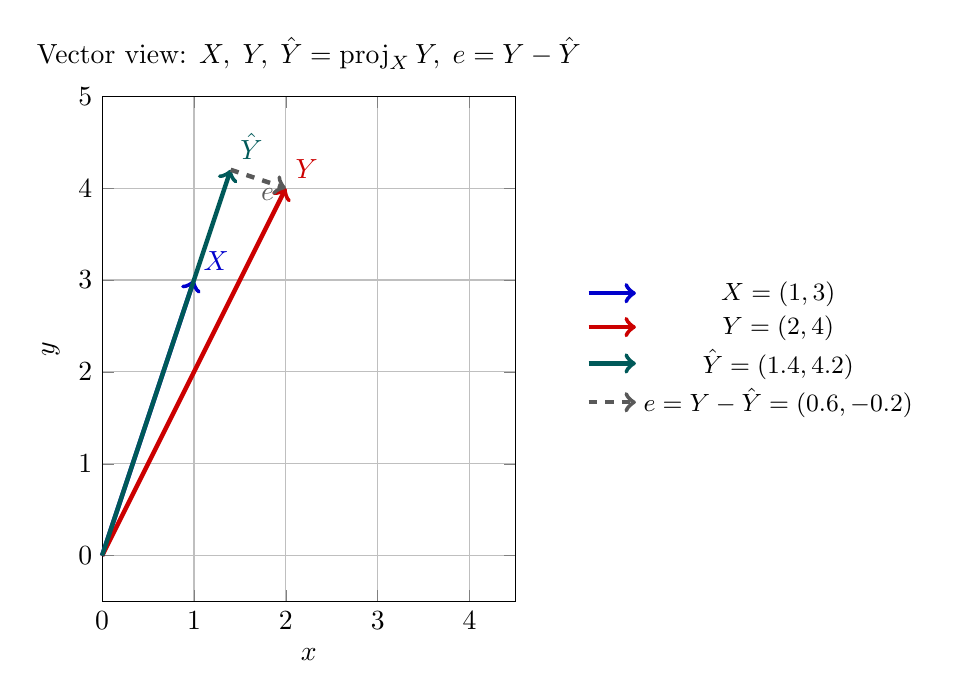
\begin{tikzpicture}
\begin{axis}[
    width=11cm, height=8cm,
    xlabel={$x$}, ylabel={$y$},
    xmin=0, xmax=4.5,
    ymin=-0.5, ymax=5,
    axis equal image,
    grid=both,
    title={Vector view: $X,\;Y,\;\hat{Y}=\operatorname{proj}_X Y,\;e=Y-\hat{Y}$},
    legend style={
        at={(1.15,0.5)}, % places legend to the right
        anchor=west,
        fill=white,
        draw=none,
        font=\small
    },
    clip=false
]

% Vectors from origin with arrowheads
\addplot[->, ultra thick, blue!80!black] coordinates {(0,0) (1,3)};       
\addlegendentry{$X=(1,3)$}

\addplot[->, ultra thick, red!80!black] coordinates {(0,0) (2,4)};       
\addlegendentry{$Y=(2,4)$}

\addplot[->, ultra thick, teal!70!black] coordinates {(0,0) (1.4,4.2)};  
\addlegendentry{$\hat{Y}=(1.4,4.2)$}

% Residual vector from \hat Y to Y (dashed with arrow)
\addplot[->, ultra thick, dashed, gray!70!black] coordinates {(1.4,4.2) (2,4)}; 
\addlegendentry{$e=Y-\hat{Y}=(0.6,-0.2)$}

% Labels near arrow tips
\node[blue!80!black, anchor=south west] at (axis cs:1,3) {$X$};
\node[red!80!black,  anchor=south west] at (axis cs:2,4) {$Y$};
\node[teal!70!black, anchor=south west] at (axis cs:1.4,4.2) {$\hat{Y}$};
\node[gray!70!black, anchor=north] at (axis cs:1.8,4.1) {$e$};

\end{axis}
\end{tikzpicture}
F

\medskip
\noindent \textbf{(d) (2 points)} In an introductory linear algebra class, you learn that the projection of vector $\vec{u}$ onto $\vec{v}$ is defined by the formula below:
\[
\operatorname{proj}_{\vec{v}}\vec{u}=\frac{\vec{u}\cdot \vec{v}}{\|\vec{v}\|^2}\,\vec{v}.
\]
Calculate the projection of $Y$ onto $X$. Which of the four vectors you plotted in (c) is equal to the projection?

\[
\operatorname{proj}_{X}Y=\frac{Y^\top X}{\|X\|^2}\,X
=\frac{14}{10}\,X
=\boxed{\hat Y}.
\]
Thus, among the four vectors from (c), the projection equals $\hat Y$.

\medskip
\noindent \textbf{(e) (2 points)} In no more than three sentences, explain the connection between the formula in Question 3, the formula provided in the introduction to Question 4, and the projection formula in part (d). How are they interrelated?

\smallskip
\noindent\textit{Answer:} In the no–intercept model we minimize $\|Y-\theta X\|^2$, and setting the derivative to zero gives 
$\hat{\theta}=\dfrac{X^\top Y}{X^\top X}$ (the result from Question 3).  
Then the fitted vector is $\hat{Y}=\hat{\theta}X=\dfrac{X^\top Y}{X^\top X}X$, which is exactly the projection formula 
$\operatorname{proj}_X Y$ from part (d).  
Thus least squares with no intercept is the orthogonal projection of $Y$ onto the span of $X$, so $e=Y-\hat{Y}$ is orthogonal to $X$.
\newpage
\noindent \textbf{(f) (1 point)} Suppose we’re interested in adding an intercept to our model. Modify your model from part (a) to plot a perfect model that achieves 0 MSE. Include the two provided points on the plot to prove that the MSE will be 0.

\noindent\textit{Answer:} Choose the line through both points:
\[
\hat y=\hat\theta_1 x+\hat\theta_0,\qquad
\hat\theta_1=\frac{4-2}{3-1}=1,\quad
\hat\theta_0=2-1\cdot 1=1.
\]
Hence the model $\boxed{\hat y=x+1}$ fits $(1,2)$ and $(3,4)$ exactly, so the training MSE is $\boxed{0}$.
\begin{figure}[h!]
    \centering
    \includegraphics[scale=0.5]{figure4_f.png}
\end{figure}

\newpage

% =======================
% Problem 5
% =======================
\newpage
\noindent\textbf{\LARGE MSE ``Minimizer''}

\medskip
\noindent \textbf{5. (8 points)} Recall from calculus that given some function $g(x)$, the $x$ you get from solving $\dfrac{dg(x)}{dx}=0$
is called a \textit{critical point} of $g$—this means it could be a minimizer or a maximizer for $g$.
In this question, we will explore some basic properties and build some intuition on why, for certain loss functions such as $L_2$ loss (squared loss), the critical point of the empirical risk function (defined as an average loss on the observed data) will always be the minimizer.

\medskip
Given some linear model $f(x)=\theta x$ for some real scalar $\theta$, we can write the empirical risk of the model $f$ given the observed data $\{(x_i,y_i)\}$, for $i\in\{1,\dots,n\}$ as the average $L_2$ loss (MSE):
\[
\frac{1}{n}\sum_{i=1}^{n}(y_i-\theta x_i)^2
=\sum_{i=1}^{n}\frac{1}{n}(y_i-\theta x_i)^2.
\]

\medskip
\noindent\textbf{(a) (3 points)} Let’s investigate one of the $n$ functions in the summation in the MSE. Define
\[
g_i(\theta)=\frac{1}{n}(y_i-\theta x_i)^2 \quad \text{for } i\in\{1,\dots,n\}.
\]
In this case, note that the MSE can be written as $\sum_{i=1}^{n} g_i(\theta)$.
Recall from calculus that we can use the 2nd derivative of a function to describe its curvature about a certain point (if it is facing concave up, down, or possibly a point of inflection). You can take the following as a fact: a function is convex if and only if the function’s 2nd derivative is non-negative on its domain. Based on this property, verify that $g_i(\theta)$ is a convex function.

\medskip
\noindent\textit{Answer:} We compute the first and second derivatives of $g_i(\theta)$:
\[
g_i'(\theta)=\frac{1}{n}\cdot 2(y_i-\theta x_i)(-x_i)
=-\frac{2x_i}{n}(y_i-\theta x_i),
\qquad
g_i''(\theta)=\frac{2x_i^2}{n}\;\ge\;0\ \ \text{for all }\theta.
\]
Since $g_i''(\theta)\ge0$ on its domain, $g_i$ is convex. (It is strictly convex if $x_i\neq0$.)

\bigskip
\noindent\textbf{(b) (3 points)} Now that we have shown that each term in the summation of the MSE is a convex function, one might wonder if the entire summation is convex, given that it is a sum of convex functions.

\smallskip
\noindent Let’s look at the formal definition of a \textbf{convex function.} Algebraically speaking, a function $g(\theta)$ is convex if, for any two points $(\theta_i,g(\theta_i))$ and $(\theta_j,g(\theta_j))$ on the function,
\[
g(c\theta_i+(1-c)\theta_j)\le c\,g(\theta_i)+(1-c)\,g(\theta_j)
\quad\text{for any } 0\le c\le 1.
\]
The function $g$ evaluated on any point between $\theta_i$ and $\theta_j$ will always lie at or below the secant line connecting $g(\theta_i)$ and $g(\theta_j)$.
\begin{figure}[h!]
    \centering
    \includegraphics[scale=0.7]{figure5_b.png}
\end{figure}
\medskip

See a graph in this Wikipedia article: \url{https://en.wikipedia.org/wiki/Convex_function}.

\smallskip
Intuitively, the above definition says that, given the plot of a convex function $g(\theta)$, if you connect two randomly chosen points on the function, the line segment will always lie on or above $g(\theta)$ (try this with the graph of $g(\theta)=\theta^2$).

\begin{enumerate}[label=\roman*.]
    \item (2 points) Using the definition above, show that if $g(\theta)$ and $h(\theta)$ are both convex functions, their sum $g(\theta)+h(\theta)$ will also be a convex function.
    \medskip\\
    \noindent\textit{Answer:} Let $g$ and $h$ be convex. For any $\theta_i,\theta_j$ and $c\in[0,1]$,
        \[
        g\!\left(c\theta_i+(1-c)\theta_j\right)
        \le c\,g(\theta_i)+(1-c)\,g(\theta_j),
        \qquad
        h\!\left(c\theta_i+(1-c)\theta_j\right)
        \le c\,h(\theta_i)+(1-c)\,h(\theta_j).
        \]
        Adding the inequalities gives
        \[
        (g+h)\!\left(c\theta_i+(1-c)\theta_j\right)
        \le c\,(g+h)(\theta_i)+(1-c)\,(g+h)(\theta_j),
        \]
        so $g+h$ is convex.

    \item (1 point) Based on what you have shown in the previous part, explain intuitively why a (finite) sum of $n$ convex functions is still a convex function when $n>2$.
    \medskip\\
    \noindent\textit{Answer:} A finite sum of convex functions is convex by repeated application of (i) (or by induction). Hence $\sum_{i=1}^n g_i$ is convex for any $n\ge2$ (and also for $n=1$).
\end{enumerate}

\medskip
\noindent\textbf{(c) (2 points)} Remember from part (a) that the MSE can be written as:
\[
\frac{1}{n}\sum_{i=1}^{n}(y_i-\theta x_i)^2=\sum_{i=1}^{n} g_i(\theta).
\]
We solve for its critical point by taking the gradient with respect to parameter $\theta$ and setting that expression to $0$. Explain why this solution is guaranteed to \emph{minimize} the MSE.
\medskip\\
\noindent\textit{Answer:}
\[
R(\theta)=\frac{1}{n}\sum_{i=1}^{n}(y_i-\theta x_i)^2=\sum_{i=1}^{n} g_i(\theta),
\]
a sum of convex functions, hence convex. Its derivative and second derivative are
\[
R'(\theta)=-\frac{2}{n}\sum_{i=1}^{n} x_i\,(y_i-\theta x_i),\qquad
R''(\theta)=\frac{2}{n}\sum_{i=1}^{n}x_i^2\ \ge\ 0.
\]
Therefore any critical point where $R'(\theta)=0$ is an absolute minimum. If not all $x_i$ are zero, then $R''(\theta)>0$ and the minimizer is unique.


% =======================
% Problem 6
% =======================
\newpage
\noindent\textbf{\LARGE Geometric Perspective of Simple Linear Regression}

\medskip
\noindent \textbf{6. (7 points)} In Lecture 12, we viewed both the simple linear regression model and the multiple linear regression model through the lens of linear algebra. The key geometric insight was that if we train a model on some design matrix $X$ and true response vector $Y$, our predicted response $\hat{Y}=X\hat{\theta}$ is the vector in $\operatorname{span}(X)$ that is closest to $Y$.

\medskip
In the simple linear regression case, our optimal vector $\theta$ is $\hat{\theta}=[\hat{\theta}_0,\hat{\theta}_1]$, and our design matrix is
\[
X=
\begin{bmatrix}
1 & x_1\\
1 & x_2\\
\vdots & \vdots\\
1 & x_n
\end{bmatrix}
=
\begin{bmatrix}
\,| & |\,\\
\mathbf{1}_n & X_{:,1}\\
\,| & |\,
\end{bmatrix}.
\]
This means we can write our predicted response vector as
\[
\hat{Y}=X
\begin{bmatrix}
\hat{\theta}_0\\
\hat{\theta}_1
\end{bmatrix}
=\hat{\theta}_0\mathbf{1}_n+\hat{\theta}_1 X_{:,1}.
\]
In this problem, $\mathbf{1}_n$ is the $n$-vector of all 1’s and $X_{:,1}$ refers to the $n$-length vector $[x_1,x_2,\dots,x_n]^\top$. Note, $X_{:,1}$ is a feature, not an observation.

\medskip
For this problem, assume we are working with the \textbf{simple linear regression model}, though the properties we establish here hold for any linear regression model that contains an intercept term.

\medskip
\noindent\textbf{(a) (3 points)} Explain why $\sum_{i=1}^{n} e_i=0$ using a geometric property. (Hint: $\vec{e}=Y-\hat{Y}$, and $\vec{e}=[e_1,e_2,\dots,e_n]^\top$. Think about how orthogonality applies here.)

\medskip
\noindent\textit{Answer:} In the OLS model, the residual vector is defined as $\vec{e}=Y-\hat{Y}$, where $\hat{Y}=X\hat{\theta}$.  
By the projection theorem, $\vec{e}$ is orthogonal to every column of $X$, meaning $X^\top \vec{e}=0$.  
Since the first column of $X$ is $\mathbf{1}_n$, we have
\[
\mathbf{1}_n^\top \vec{e}=0
\quad\Longrightarrow\quad
\sum_{i=1}^n e_i = 0.
\]
Thus, the sum of all residuals is zero.

\medskip
\noindent\textbf{(b) (2 points)} Similarly, explain why $\sum_{i=1}^{n} e_i x_i=0$ using a geometric property. (Hint: Your answer should be very similar to the above.)

\medskip
\noindent\textit{Answer:}
Again, because $\vec{e}$ is orthogonal to \emph{each} column of $X$, it must also be orthogonal to the second column $X_{:,1} = [x_1, x_2, \dots, x_n]^\top$.  
Therefore,
\[
X_{:,1}^\top \vec{e}=0
\quad\Longrightarrow\quad
\sum_{i=1}^n e_i x_i = 0.
\]
Hence, the weighted sum of residuals with respect to $x_i$ is zero.
\medskip
\\\noindent\textbf{(c) (2 points)} Briefly explain why the vector $\hat{Y}$ must also be orthogonal to the residual vector $\vec{e}$.
\medskip
\\\noindent\textit{Answer:} In OLS, $\hat{Y}=X\hat{\theta}$ lies entirely within $\text{span}(X)$, the column space of $X$,  
and the residual vector $\vec{e}=Y-\hat{Y}$ lies in the orthogonal complement of that space.  
Since these two subspaces are perpendicular, it follows that
\[
\hat{Y}^\top \vec{e}=0,
\]
meaning the predicted response vector $\hat{Y}$ is orthogonal to the residuals $\vec{e}$.
% =======================
% Problem 7
% =======================
\newpage
\noindent\textbf{\LARGE A Special Case of Linear Regression}

\medskip
\noindent \textbf{7. (8 points)} In this question, we fit a model:
\[
y^{O}=\theta^{O}_0+\theta^{O}_1 x_1+\theta^{O}_2 x_2
\]
using $L_2$ loss. The superscript $O$ is used to denote an Ordinary Least Squares (OLS) model with two features.

\medskip
The data are given below:
\[
\begin{array}{c|ccc}
\mathbb{Y}  & \text{bias} & \mathbb{X} _{:,1} & \mathbb{X} _{:,2}\\ \hline
-1 & 1 & 1  & 1\\
 3 & 1 & -2 & 0\\
 4 & 1 & 1  & -1
\end{array}
\]

\medskip
\noindent\textbf{(a) (3 points)} Find
\[
\hat{\theta}^{O}=
\begin{bmatrix}
\hat{\theta}^{O}_0\\
\hat{\theta}^{O}_1\\
\hat{\theta}^{O}_2
\end{bmatrix}
\]
using the formula derived in lecture 12:
\[
\hat{\theta}^{O}=(X^\top X)^{-1}X^\top Y.
\]
Explicitly write out the matrix $X$ for this problem and \textbf{show all steps.}
\medskip
\\\noindent\textit{Answer:}
The design matrix and response vector are
\[
X=
\begin{bmatrix}
1 & \phantom{-}1 & \phantom{-}1\\
1 & -2 & \phantom{-}0\\
1 & \phantom{-}1 & -1
\end{bmatrix},
\qquad
Y=\begin{bmatrix}-1\\3\\4\end{bmatrix}.
\]
Compute
\[
X^\top X=
\begin{bmatrix}
3 & 0 & 0\\
0 & 6 & 0\\
0 & 0 & 2
\end{bmatrix},
\qquad
X^\top Y=
\begin{bmatrix}
6\\[2pt]-3\\[2pt]-5
\end{bmatrix}.
\]
Finding the inverse of $X^\top X$ is straightforward since it is diagonal:
\[
(X^\top X)^{-1}=
\begin{bmatrix}
\frac13 & 0 & 0\\[2pt]
0 & \frac16 & 0\\[2pt]
0 & 0 & \frac12
\end{bmatrix},
\quad
\Rightarrow\quad
\hat\theta^{O}
=(X^\top X)^{-1}X^\top Y
=
\begin{bmatrix}
2\\[2pt]
-\tfrac12\\[2pt]
-\tfrac52
\end{bmatrix}.
\]

\medskip
\noindent\textbf{(b) (2 points)} Mathematically show that MSE for the OLS is 0. Additionally, give a geometric explanation as to why the MSE is 0. (As a sanity check, the sum of residuals should be 0.)
\medskip
\\\noindent\textit{Answer:}
Using $\hat\theta^{O}$ from part (a), we compute the predictions and MSE:
\smallskip
\\\noindent Predictions:
\[
\hat Y=X\hat\theta^{O}
=
\begin{bmatrix}
1 & \phantom{-}1 & \phantom{-}1\\
1 & -2 & \phantom{-}0\\
1 & \phantom{-}1 & -1
\end{bmatrix}
\begin{bmatrix}
2\\ -\tfrac12\\ -\tfrac52
\end{bmatrix}
=
\begin{bmatrix}
-1\\[2pt]3\\[2pt]4
\end{bmatrix}
=Y.
\]
Thus the residual vector $e=Y-\hat Y=\mathbf{0}$ and
\[
\text{MSE}=\frac1n\sum_{i=1}^n (y_i-\hat y_i)^2
=\frac13\|e\|_2^2
=0.
\]
\textit{Geometric view:} $X$ is $3\times3$ with $\det(X)=6\neq0$, so its columns span $\mathbb{R}^3$. Therefore $Y\in\mathrm{span}(X)$ and the orthogonal projection of $Y$ onto $\mathrm{span}(X)$ equals $Y$ itself, giving zero residual.
\medskip

\noindent\textbf{(c) (3 points)} Instead of using $X_{:,2}$ as a feature in our second model, we decided to transform it and use $X_{:,2}^2$ instead. That is, the dataset we use is modified as follows:
\[
\begin{array}{c|ccc}
\mathbb{Y}  & \text{bias} & \mathbb{X} _{:,1} & \mathbb{X} _{:,2}^2\\ \hline
-1 & 1 & 1  & 1^2=1\\
 3 & 1 & -2 & 0^2=0\\
 4 & 1 & 1  & (-1)^2=1
\end{array}
\]
Accordingly, we calculate a single prediction using the new model as specified below:
\[
y_{\text{new}}=\theta^{\text{new}}_0+\theta^{\text{new}}_1 x_1+\theta^{\text{new}}_2 x_2^2.
\]
Is it possible to find a unique optimal solution in this case? If so, compute $\hat{\theta}^{\text{new}}$ and the corresponding value of MSE. If not, explain why this is not possible. Regardless of which way you answer, similar to part (a), explicitly write out the matrix $X_{\text{new}}$ for this problem and \textbf{show all steps.}

\medskip
\noindent\textit{Answer:} The design matrix and response vector are:
\[
X_{\text{new}} =
\begin{bmatrix}
1 & 1 & 1\\
1 & -2 & 0\\
1 & 1 & 1
\end{bmatrix},
\qquad
Y =
\begin{bmatrix}
-1\\
3\\
4
\end{bmatrix}.
\]

\noindent
We can see that the \textbf{second column is a linear combination of the first and third columns}. Specifically,
\[
\text{col}_2 = -2 \cdot \text{col}_1 + 3 \cdot \text{col}_3.
\]
This implies the columns of $X_{\text{new}}$ are linearly dependent.

\medskip
\noindent In other words, there exists a nonzero vector
\[
v =
\begin{bmatrix}
2\\[2pt]
1\\[2pt]
-3
\end{bmatrix}
\quad \text{such that} \quad
X_{\text{new}} v = 0.
\]
Therefore,
\[
\operatorname{rank}(X_{\text{new}}) = 2
\quad\text{and}\quad
X_{\text{new}}^{\top} X_{\text{new}}\ \text{is not invertible.}
\]

\medskip
\noindent Because $X_{\text{new}}$ is not full column rank, there are infinitely many parameter vectors $\hat{\theta}^{\text{new}}$ that minimize the loss function and yield the same fitted values. Thus, the OLS solution is not unique, and we cannot compute a single inverse for $(X_{\text{new}}^{\top} X_{\text{new}})$.

\textbf{\\
\\
\\
\\
\\
\\
\\
\\
\\
\\
}


\begin{center}
    \textbf{\Large Congratulations!}\\[6pt]
    You have finished Homework 5!
\end{center}

Hii reader I spent way too long formatting latex on this homework. Please give me a 100 :(

\end{document}
